% !TEX TS-program = xelatex
% !TEX encoding = UTF-8 Unicode

% This is a simple template for a LaTeX document using the "article" class.
% See "book", "report", "letter" for other types of document.

\documentclass[11pt]{article}

\usepackage[margin=1in]{geometry}
\usepackage{fancyhdr}
\usepackage{framed}
\usepackage{amsmath,amsthm,amssymb}

\usepackage{titlesec}

\usepackage[svgnames]{xcolor}

\usepackage{enumerate}

%\usepackage{mathpazo}
\usepackage{mathtools}
\usepackage{unicode-math}

\usepackage{xunicode} %handle unicode
\usepackage{xltxtra} %XeTeX extras
\usepackage{fontspec} %use OTF/TTF fonts


%\newcommand{\lmr}{\fontfamily{lmr}\selectfont} % Latin Modern Roman


%\setmainfont{Myriad Pro} %use this font
%\setmathfont{Adobe Garamond Pro} %use this font for math

\titleformat{\section}
  {\large\bf}{\thesection}{0.25em}{}[\titlerule]
\titlespacing{\section}
  {0pt}{*1.5}{0.25em}

\titleformat{\subsection}
  {\normalfont\bf}{\thesubsection}{0.25em}{}
\titlespacing{\subsection}
  {0pt}{*1}{0.125em}

\renewcommand\thesection{\Alph{section}}

\renewcommand{\labelitemi}{\textemdash}

\DeclareMathOperator{\dif}{d\!}
%\DeclareMathOperator{\Pr}{P}
\DeclareMathOperator{\E}{E}
\DeclareMathOperator{\var}{var}
\DeclareMathOperator{\F}{\mathfrak{F}}
\DeclareMathOperator{\Poisson}{Poisson}
\DeclareMathOperator{\Bernoulli}{Bernoulli}
\DeclareMathOperator{\Binomial}{Binomial}
\DeclareMathOperator{\Order}{O}
\DeclareMathOperator{\Uniform}{Uniform}


\newenvironment{propertybox}{%
   \def\FrameCommand{\colorbox{LightSteelBlue}}%
   \MakeFramed{\advance\hsize-\width \FrameRestore}}
 {\endMakeFramed}

\lhead{\textbf{ELEC548}}
\chead{Byron's Review of Poisson Processes}
\cfoot{}
\rhead{}
\rfoot{\thepage}
\pagestyle{fancyplain}

\setlength\parindent{0pt}

\begin{document}
\setmainfont{Myriad Pro} %use this font
%\setmathfont{Latin Modern Math}
\setmathfont[Path = /usr/share/texmf/fonts/opentype/public/tex-gyre-math/,Extension=.otf]{texgyrepagella-math}
%\setmathfont{TG Pagella Math}

\begin{center}
\large
\textbf{ELEC 548} Byron's Review of Poisson Processes
\end{center}

\section{Exponential Distribution}
A random variable $T$ is said to be exponentially distributed with rate $\lambda > 0$ if its probability
density function (PDF) is
\begin{equation}
f_T(t) = \begin{cases} \lambda e^{-\lambda t} & \text{if} \quad t \geq 0 \\ 0 & \text{if} \quad t \leq 0. \end{cases}
\end{equation}
As a shorthand, we can write $T \sim \exp(\lambda)$.

\begin{center}
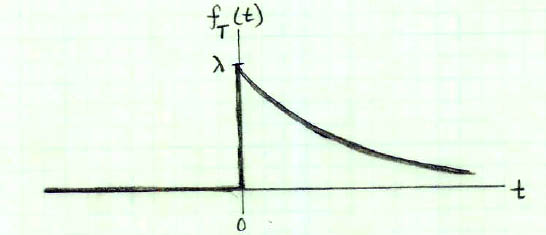
\includegraphics[scale=0.5]{Figure1.jpg}
\end{center}

{\bf A peak ahead:} The time between two consecutive spikes (a.k.a. the inter-spike interval or ISI) can be modeled by an
exponential distribution.

Alternatively, we can describe $T$ in terms of its cumulative distribution function (CDF).
\begin{equation}
F_T(t) = \Pr (T \leq t) = \begin{cases} 1 - e^{-\lambda t} & \text{if} \quad t \geq 0 \\ 0 & \text{if} \quad t \leq 0. \end{cases}
\end{equation}

\begin{center}
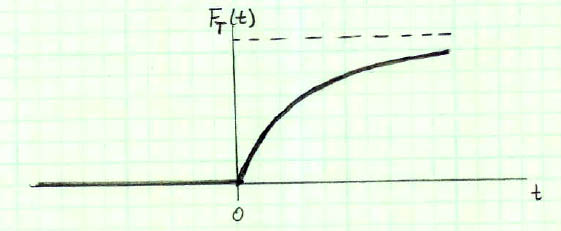
\includegraphics[scale=0.5]{Figure2.jpg}
\end{center}

\begin{framed}
Note that the PDF and CDF (of any random variable) are related in the following way:
\begin{equation}
f_T(t) = \frac{\dif F_T(t)}{\dif t} \quad \quad F_T(t) = \int^{t}_{-\infty} f_T(t) \, \dif t
\end{equation}
\end{framed}

\subsection{Mean and variance of the exponential}
\begin{equation}
\begin{split}
\E[T] &= \int t f_T(t) \dif t \\
   &= \int_0^{\infty} t \, \lambda e^{-\lambda t} \dif t
\end{split}
\end{equation}
Integrating by parts; let $u=t$ and $\dif v = \lambda e^{-\lambda t}$, 
    so $\dif u= \dif t$ and $v = -e^{-\lambda t}$.
\begin{equation}
\begin{split}
\E[T] &= u v \rvert_0^{\infty} - \int_0^{\infty} v du \\
   &= -t \, e^{-\lambda t} \rvert_0^{\infty} + \int_0^{\infty} e^{-\lambda t} \dif t \\
   &= 0 - 0 + \left[-\frac{1}{\lambda} e^{-\lambda t}\right]_0^{\infty} \\
   &= \frac{1}{\lambda}
\end{split}
\end{equation}

\begin{equation}
\begin{split}
\E[T^2] &= \int t^2 f_T(t) \dif t \\
   &= \int_0^{\infty} t^2 \, \lambda e^{-\lambda t} \dif t
\end{split}
\end{equation}
Integrating by parts; let $u=t^2$ and $\dif v = \lambda e^{-\lambda t}$, 
    so $\dif u= 2 t \dif t$ and $v = -e^{-\lambda t}$.
\begin{equation}
\begin{split}
\E[T^2] &= u v \rvert_0^{\infty} - \int_0^{\infty} v du \\
   &= -t^2 \, e^{-\lambda t} \rvert_0^{\infty} + \int_0^{\infty} 2 t e^{-\lambda t} \dif t \\
   &= 0 - 0 +  \int_0^{\infty} 2 t e^{-\lambda t} \dif t\\
   &= \frac{2}{\lambda} \int_0^{\infty} \lambda t e^{-\lambda t} \dif t\\
   &= \frac{2}{\lambda^2}
\end{split}
\end{equation}
and
\begin{equation}
\var(T) = \E(T^2) - \left(E[T]\right)^2 = \frac{1}{\lambda^2}
\end{equation}

\subsection{Memoryless property of exponential random variables}

{\bf In words:} Say that the waiting time for a bus to arrive is exponentially distributed. If I've been waiting
for $t$ seconds, then the probability that I must wait $s$ more seconds is the same as if I hadn't waited
at all.

{\bf With math:}
\begin{equation}
\Pr\left(T > t + s \vert T > t\right) = \Pr\left(T > s\right)
\end{equation}
To show this,
\begin{equation}
\Pr\left(T > t + s \vert T > t\right) = \frac{\Pr\left(T > t + s\right)}{\Pr\left(T > t\right)}
\end{equation}

{\it Intuition:} Conditioning the exponential is like starting at a point away from zero on the
x axis of the PDF. Turning that new thing into a distribution implies renormalizing, but because 
of an exponential's shape, that stretching turns it into exactly the same thing as it was before.

\section{Defining the Poisson process}
\subsection{Constructing a Poisson process}
Let $t_1, t_2, \ldots$ be independent exponential random variables with parameter $\lambda$. Let
$T_n = t_1 + t_2 + \ldots + t_n$ for $n \geq 1$, where $T_0 = 0$. Define $N(s) = \max \lbrace n : T_n \leq s\rbrace$. $N(s)$ is a Poisson process.

\begin{center}
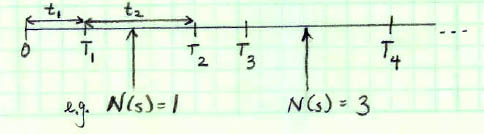
\includegraphics[scale=0.5]{Figure3.jpg}
\end{center}

If a Poisson process is used to model a spie train, then:
\begin{itemize}
\item $t_n$ is the $n^{\text{th}}$ interspike interval (ISI).
\item $T_n$ is the time at which the $n^{\text{th}}$ spike occurs.
\item $N(s)$ is the number of spikes by time $s$.
\end{itemize}


\subsection{Properties of the Poisson process}
Why is $N(s)$ called a Poisson process rather than an exponential process?

\begin{propertybox}
{\bf Property 1:} $N(s)$ has a Poisson distribution with mean $\lambda s$.
\end{propertybox}

First, recognize that $N(s)=n$ iff $T_n \leq s < T_{n+1}$. In other words, the $n^{\text{th}}$ spike
occurs \emph{before} time $s$ and the $(n+1)^{\text{th}}$ spike occurs \emph{after} time $s$.

\begin{equation*}
\begin{split}
\Pr\left(N(s) = n\right) &= \int_0^s \Pr\left(T_{n+1} > s \vert T_n = t\right) f_{T_n}(t) \dif t \\
  &= \int_0^s \Pr\left(t_{n+1} > s-t\right) f_{T_n}(t) \dif t \\
  &= \int_0^s e^{-\lambda (s - t)} f_{T_n}(t) \dif t
\end{split}
\end{equation*}

Recall that summing independent random variables implies convolving their PDF's. If we take Fourier transforms of the PDF's, then we can multiply rather than convolve.
\begin{equation*}
\begin{split}
\F\lbrace f_{T_n} \rbrace &= \prod_{i=1}^{n} \F \lbrace f_{T_i} \rbrace \\
  &= \left[\F \lbrace \lambda e^{-\lambda t} u(t)\rbrace \right]^n \\
  &= \left[ \frac{\lambda}{\lambda + \jmath \omega} \right]^n
\end{split}
\end{equation*}

\begin{center}
\fbox{\begin{minipage}{0.4\linewidth}
Table of Fourier Transforms
\begin{equation*}
e^{-a t} u(t) \xrightarrow{\F} \frac{1}{a + \jmath \omega}
\end{equation*}
\begin{equation*}
t^n e^{-a t} u(t) \xrightarrow{\F} \frac{n!}{\left(a + \jmath \omega\right)^{n+1}}
\end{equation*}
\end{minipage}}
\end{center}

Taking the inverse transforms of both sides,
\begin{equation}
\begin{split}
f_{T_n}(t) &= \frac{\lambda^n}{\left(n-1\right)!} \cdot t^{n-1} e^{-\lambda t} u(t) \\
  &= \lambda e^{-\lambda t} \frac{ \left(\lambda t\right)^{n-1}}{\left( n-1\right)!} \quad \text{for}
     \, t \geq 0
\end{split}
\end{equation}

This is called the {\bf Erlang distribution} which is a special case of the {\bf gamma distribution}.
This will appear again when we try to model refractory periods.


\begin{equation*}
\begin{split}
\Pr\left(N(s) = n\right)  &= \int_0^s e^{-\lambda (s - t)} f_{T_n}(t) \dif t \\
 &= \int_0^s e^{-\lambda (s - t)} \lambda e^{-\lambda t} \frac{ \left(\lambda t\right)^{n-1}}{\left( n-1\right)!}  \dif t \\
 &=  \frac{\lambda^n}{\left( n-1\right)!} e^{-\lambda s}  \int_0^s t^{n-1}  \dif t \\
 &=  \frac{\lambda^n}{\left( n-1\right)!} e^{-\lambda s}  \left[\frac{t^n}{n}\right]_0^s \\
 &=  e^{-\lambda s} \frac{\left(\lambda s\right)^n}{n!}  = \Poisson(\lambda s)
\end{split}
\end{equation*}

What does a Poisson distribution look like? 

\begin{center}
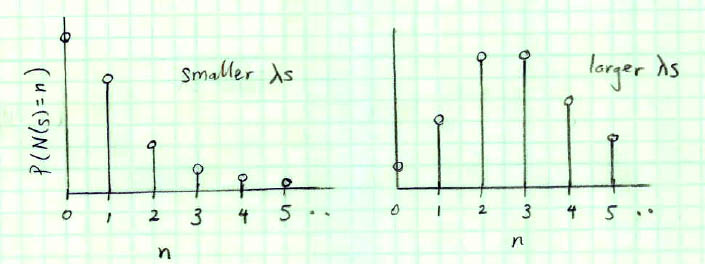
\includegraphics[scale=0.5]{Figure4.jpg}
\end{center}


For smaller $(\lambda s)$, the exponential term dominates. For larger
$(\lambda s)$, the polynomial term initially dominates.

What are the mean and variance of the Poisson distribution? First the mean:
\begin{equation}
\begin{split}
\E\left[ N(s)\right] &= \sum_{n=0}^{\infty} n \cdot \Pr\left(N(s) = n\right) \\
  &= \sum_{n=1}^{\infty} n \cdot e^{-\lambda s} \frac{(\lambda s)^n}{n!} \\
  &= \lambda s \sum_{n=1}^{\infty} e^{-\lambda s} \frac{ (\lambda s)^{n-1} }{(n-1)!} \\
  &= \boxed{\lambda s}
\end{split}
\end{equation}
For the variance, we can use a trick.
\begin{equation}
\begin{split}
\E\left[ N(s) \left(N(s) - 1\right)\right] &= \sum_{n=0}^{\infty} n (n-1) \cdot \Pr\left(N(s) = n\right) \\
  &= \sum_{n=2}^{\infty} n (n - 1) \cdot e^{-\lambda s} \frac{(\lambda s)^n}{n!} \\
  &= (\lambda s)^2 \sum_{n=2}{\infty} e^{-\lambda s} \frac{ (\lambda s)^{n-2} }{(n-2)!} \\
  &= (\lambda s)^2.
\end{split}
\end{equation}
\begin{equation}
\begin{split}
\var\left[ N(s) \right] &= \E\left[N(s)^2\right] - \left(\E\left[N(s)\right]\right)^2 \\
  &= \E\left[ N(s) \left( N(s) - 1\right)\right] + \E\left[ N(s) \right] - \left(\E\left[N(s)\right]\right)^2 \\
  &= (\lambda s)^2 + \lambda s - (\lambda s)^2 \\
  &= \boxed{\lambda s}
\end{split}
\end{equation}

\begin{propertybox}
{\bf Property 2:}
$N(t+s) - N(s), \, t\geq 0, \, \sim \Poisson(\lambda t)$ and independent of $N(r), \, 0\leq r \leq s$.
\end{propertybox}
In other words, if you look forward from any time s, that is itself a Poisson process independent of anything that's already
happened. This picture provides the intuition:

\begin{center}
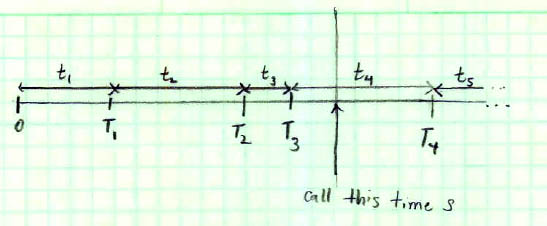
\includegraphics[scale=0.5]{Figure5.jpg}
\end{center}

Looking forward from time $s$, the time until the first spike (at $T_4$) is distributed as an exponential with parameter $\lambda$
and independent of anything that came before it, by the memoryless property of the exponential. Subsequent ISI's
($t_5, t_6, \ldots$) are $\sim \exp (\lambda)$ and independent of anything before time $s$.

\begin{propertybox}
{\bf Property 3:} $N(t)$ has \underline{independent increments}.
\end{propertybox}

\begin{multline*}
\text{If } s_0 < s_1 < \ldots < s_n, \text{then} \\
N(s_1) - N(s_0), N(s_2) - N(s_1), \ldots, N(s_n) - N(s_{n-1})
\text{ are independent}.
\end{multline*}

In other words, if you take spike counts in non-overlapping windows, the spike counts are independent.

\begin{center}
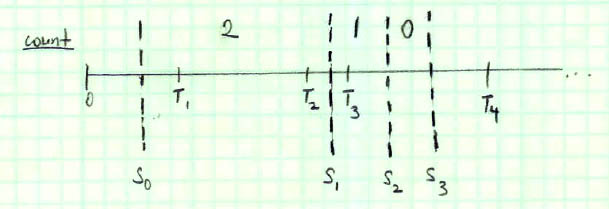
\includegraphics[scale=0.5]{Figure6.jpg}
\end{center}

\begin{propertybox}
{\bf To summarize,} if $N(s), s\geq0$ is a Poisson process, then
\begin{enumerate}[(i)]
\item \label{Prop1} $N(0) = 0$
\item \label{Prop2} $N(t + s) - N(s) \sim \Poisson(\lambda t)$
\item \label{Prop3} $N(t)$ has indepdent increments
\end{enumerate}
Conversely if \ref{Prop1}, \ref{Prop2}, and \ref{Prop3} hold, then $N(s), s\geq0$ is a Poisson process.
\end{propertybox}

\subsection{Another view of the Poisson process}
So far, we have derived the Poisson process using i.i.d. exponential ISI's. Another very useful way of thinking about
the Poisson process is using the Bernoulli process. The Poisson process is the continuous-time limit of the Bernoulli
process, which is defined in discrete time.

{\bf Bernoulli Process}

At each time step, flip a coin to decide whether the neuron spikes (1) or not (0). The coin flips are independent of each
other.

\begin{center}
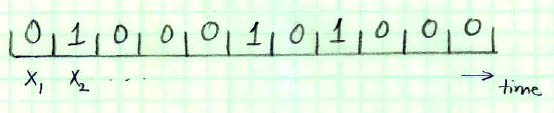
\includegraphics[scale=0.5]{Figure7.jpg}
\end{center}

At the $i^{\text{th}}$ time step,
\begin{gather*}
X_i \sim \Bernoulli (p) \text{ i.i.d.} \\
X_i = \begin{cases} 1 & \text{with probability }  \, p \\ 0 & \text{with probability }  \, (1-p) \end{cases}
\end{gather*}
Let $S_n$ be the number of spikes up to and including the $n^{\text{th}}$ time step.
\begin{gather*}
S_n = \sum_{i=1}^n X_i \\
S_n \sim \Binomial(n,p) \\
\Pr(S_n = k) = \binom{n}{k} p^k \left(1-p\right)^{n-k} \\
\E[S_n] = np \Rightarrow \text{We expect to see $n p$ spikes in $n$ time steps.}
\end{gather*}

Without proof here, as $n \rightarrow \infty$ and $p \rightarrow 0$, the Bernoulli process becomes the Poisson process, where
 $n p = \lambda s$. So the Bernoulli process provides an intuitive way to think about the Poisson process.

We can also go in the other direction and consider the probability that a Poisson process gives a spike in a small
time window of duration $\delta$. The number of spikes in this window is $\sim \Poisson(\lambda \delta)$.
\begin{gather*}
\Pr\left(0 \text{ spikes in } [t, t + \delta]\right) = e^{-\lambda \delta} = \boxed{1 - \lambda \delta} + \Order(\delta^2) \\
\Pr\left(1 \text{ spikes in } [t, t + \delta]\right) = e^{-\lambda \delta} \cdot \lambda \delta = \boxed{\lambda \delta} - \Order(\delta^2) \\
\Pr\left( >1 \text{ spikes in } [t, t + \delta]\right) = e^{-\lambda \delta} = \Order(\delta^2)
\end{gather*}
If $\delta$ is small, $\Order(\delta^2)$ terms $\rightarrow 0$. Thus, whether or not a neuron spikes in this small window can
be determined with a coin flip, where the probability of a spike is $\lambda \delta$.

\subsection{Thinning}
Suppose $N(s)$ is a Poisson process with rate $\lambda$. Each time a spike occurs, a coin is flipped. If the coin comes up
heads (with probability $p$), the spike is assigned to output stream 1. Else, the spike is assigned to output stream 2. The two
output streams are each an independent Poisson process with rates $\lambda p$ and $\lambda (1-p)$, respectively.

\begin{center}
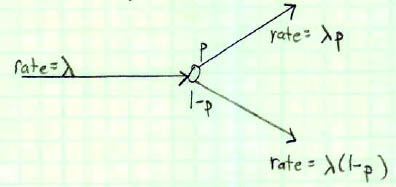
\includegraphics[scale=0.5]{Figure8.jpg}
\end{center}

\subsection{Superposition}
Suppose $N_1(s)$ and $N_2(s)$ are independent Poisson processes with rates $\lambda_1$ and $\lambda_2$, respectively. Then
$N_1(s) + N_2(s)$ is a Poisson process with rate $\lambda_1 + \lambda_2$.

\begin{center}
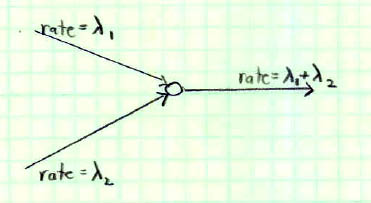
\includegraphics[scale=0.5]{Figure9.jpg}
\end{center}

\section{Inhomogeneous Poisson Processes}
So far, we've considered a Poisson process that is homogeneous -- it's rate does not change as a function of time. However,
the firing rates of neurons typically \underline{do} change with time. To model the time-dependent activity of neurons, we need
a non-stationary process, such as the \emph{inhomogeneous} Poisson process.

\begin{propertybox}
{\bf Definition} $N(s), s \geq 0$ is an inhomogeneous Poisson process with rate $\lambda(r)$ if
\begin{enumerate}[(i)]
\item $N(0) = 0$
\item $N(t + s) - N(s) \sim \Poisson(\int_s^{t+s} \lambda(r) \dif r)$
\item $N(t)$ has indepdent increments
\end{enumerate}
\end{propertybox}
Comparing with the previous definition of a homogeneous Poisson process, the only difference is that the Poisson mean is now
$\int_s^{t+s} \lambda(r) \dif r$ rather than $\lambda t$.

Note that if $\lambda(r)$ is flat, then the two definitions are equivalent!

\begin{center}
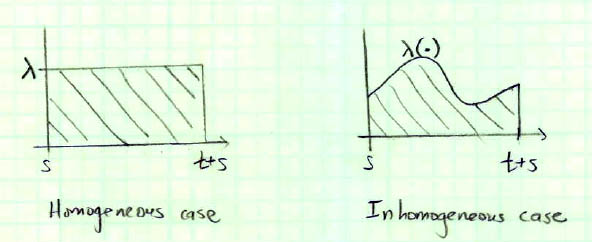
\includegraphics[scale=0.5]{Figure10.jpg}
\end{center}

For an inhomogeneous Poisson process, the ISI's are \underline{no longer} exponentially distributed or independent. Let's show this:

\begin{center}
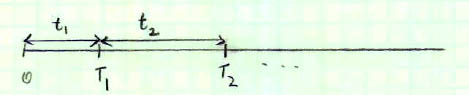
\includegraphics[scale=0.5]{Figure11.jpg}
\end{center}

\begin{gather*}
\text{Let } \mu(t) = \int_0^t \lambda(r) \dif r \\
\Pr(t_1 > t) = \Pr\left(N(t) = 0\right) = e^{-\int_0^t \lambda(r) \dif r} = e^{-\mu(t)} \\
f_{t_1} = -\frac{\dif}{\dif t} \Pr(t_1 > t) = \lambda(t) e^{-\mu(t)}, \text{ which is not exponential!}
\end{gather*}

Now, look forward in time from $T_1$.
\begin{align*}
\Pr(t_2 > s \vert t_1=t) &= \Pr\left(N(t+s) - N(t) = 0\right) \\
 &= e^{-\int_t^{t+s} \lambda(r) \dif r} \\
 &= e^{-(\mu(s+t)  - \mu(t))}
\end{align*}
\begin{equation*}
f_{t_2 \vert t_1} (s) = -\frac{\dif}{\dif s} \Pr(t_s > s \vert t_1 = t) = \lambda(s + t) e^{-(\mu(s+t)  - \mu(t))}
\end{equation*}
Since $t_2$ depends on $t_1$, the ISIs are not independent. 

The joint distribution of ISI's is
\begin{align*}
f_{t_1,t_2}(t,s) &= f_{t_2 \vert t_1} (s) \cdot f_{t_1} (t) \\
 &= \lambda(t) \lambda(s + t) e^{-\mu(s+t)}.
\end{align*}
Changing variables from ISI's to spike times (i.e., $\nu_1 = t$, $\nu_2 = s + t$),
\begin{equation*}
f_{T_1,T_2}(\nu_1,\nu_2) = \lambda(\nu_1) \lambda(\nu_2) e^{-\mu(\nu_2)}.
\end{equation*}
For more than two spikes, we get
\begin{equation}
\label{spike_train_density}
\boxed{f_{T_1,\ldots,T_n}(\nu_1,\ldots,\nu_n) = \lambda(\nu_1) \ldots \lambda(\nu_n) e^{-\mu(\nu_n)}}.
\end{equation}
\emph{Sanity check:} What does the spike train probability density \ref{spike_train_density} reduce down to
for a homogeneous Poisson process?

For a homogeneous Poisson process, $\lambda (r) = \lambda_0 \forall r$. So,
\begin{equation}
\label{homogeneous_spike_train}
f_{T_1,\ldots,T_n}(\nu_1,\ldots,\nu_n) = \lambda_0^n e^{-\lambda_0 \nu_n}.
\end{equation}
Note that this does not depend on the spike times $\nu_1, \ldots, \nu_{n-1}$. Given that $n$ spikes occured and the
time of the last spike $\nu_n$, all spike trains have the sam probability. Equation \ref{homogeneous_spike_train} could also
have been obtained by multiplying exponential distributions, since ISI's are i.i.d.
\begin{align*}
f_{t_1,\ldots,t_n}(u_1,\ldots,u_n) &= \prod_{i=1}{n} \lambda_0 e^{-\lambda_0 u_i} \\
 &= \lambda_0^n e^{-\lambda_0 \left(\sum_{i=1}^n u_i\right)}
\end{align*}
where $\nu_n = \sum_{i=1}^n u_i$.

\section{Generating Poisson processes}
\begin{center}
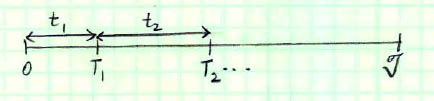
\includegraphics[scale=0.5]{Figure12.jpg}
\end{center}
\subsection{Homogeneous Poisson process with rate $\lambda$}
\underline{Method 0} (Note - this is the most inefficient method!)
\begin{itemize}
\item Pick a bin size $\Delta t$ such that $\left(1 - (1 + \lambda \Delta t) e^{-\lambda \Delta t}\right) \approx 0$ 
(i.e., the probability that more than one spike is emitted in a bin is very small).
\item Generate a vector of $\Uniform([0 1])$ random variables, $U_1, \ldots, U_M,$ where $M = \lceil \frac{\mathcal{T}}{\Delta t} \rceil$. 
(In  {\sc Matlab} use ``{\tt rand}''.)
\item Emit a spike in bin $m$ if $U_m < \lambda \Delta t$, with corresponding spike time $T_k = m \Delta t$.
\end{itemize}
\underline{Method 1}
\begin{itemize}
\item Generate i.i.d. exponential random variables $t_1, t_2, \ldots$ with parameter $\lambda$. (In {\sc Matlab} use
``{\tt exprnd}''.)
\item The spike times are $T_n = \sum_{i=1}^n t_i$
\item If $T_n > \mathcal{T}$, stop
\end{itemize}

\underline{Method 2}
\begin{itemize}
\item Draw $N \sim \Poisson(\lambda \mathcal{T})$, the number of spikes on the interval $[0, \mathcal{T}]$. (In {\sc Matlab} 
use ``{\tt poissrnd}''.)
\item Draw $T_1, \ldots, T_N \sim \Uniform([0, \mathcal{T})$. (In  {\sc Matlab} use ``{\tt rand}''.) The $T_1, \ldots, T_n$ are
the spike times. (Cool!)
\end{itemize}
\begin{framed}
\emph{Why does Method 2 work?} \\
The intuition is that a spike should not be more likely to occur at one time compared to another time (think of a Bernoulli process).
More formally, Method 2 is based on the following (not-proved-here) theorem:
\begin{propertybox}
{\bf Theorem:} If we conditionon $N(\mathcal{T}) = M$, then the set of spike times $\lbrace T_1,\ldots,T_M\rbrace$ has the
same distribution as $\lbrace U_1,\ldots,U_M\rbrace$, where $U_1, \ldots, U_M \sim \Uniform\left([0, \mathcal{T}]\right)$ i.i.d.
\end{propertybox}
\end{framed}

\subsection{Inhomogeneous Poisson process with rate $\lambda (t)$}
\underline{Method 0}
See Method 0 above.

\underline{Method 1}
\begin{itemize}
\item Let $\lambda_{\max} = \underset{t}{\max} \, \lambda(t)$. Generate a \underline{homogeneous} Poisson process with rate
$\lambda_{\max}$ using one of the methods above.
\item For $n = 1, \ldots, N$
\begin{equation*}
\begin{rcases} \text{Draw } U \sim \Uniform([0, 1]) \\ \text{If } U > \frac{\lambda(T_n)}{\lambda_{\max}} 
   \text{ reject the spike at } T_n \quad \\ \text{Else, retain the spike at } T_n.\end{rcases} \text{thinning} 
\end{equation*}
\end{itemize}
The spikes that are retained at the end of this procedure represent an inhomogeneous Poisson process with rate $\lambda(t)$.

\end{document}


